% 版式与封面：Pandoc PDF 构建
\usepackage[a4paper,margin=2.1cm,top=2.35cm,bottom=2.15cm]{geometry}
\usepackage{graphicx}
\usepackage{booktabs}
\usepackage{longtable}
\usepackage{array}
\usepackage{calc}
\usepackage{etoolbox}
\usepackage{fancyhdr}
\usepackage{titlesec}
\usepackage{enumitem}
\usepackage{xcolor}
\usepackage{newunicodechar}
\usepackage{amssymb}

\definecolor{towersoulsteal}{HTML}{177E7A}
\definecolor{towersoulsdark}{HTML}{0B2B33}
\definecolor{towersoulsgold}{HTML}{B8862B}

\setlength{\parindent}{0pt}
\setlength{\parskip}{4pt}
\setlist{itemsep=2pt,topsep=3pt,leftmargin=1.5em}
\AtBeginEnvironment{longtable}{\footnotesize}
\setkeys{Gin}{width=\linewidth,height=0.43\textheight,keepaspectratio}

\newunicodechar{→}{\ensuremath{\rightarrow}}
\newunicodechar{↔}{\ensuremath{\leftrightarrow}}
\newunicodechar{×}{\ensuremath{\times}}
\newunicodechar{≤}{\ensuremath{\leq}}
\newunicodechar{≥}{\ensuremath{\geq}}
\newunicodechar{✓}{\ensuremath{\checkmark}}
\newunicodechar{✔}{\ensuremath{\checkmark}}
\newunicodechar{▤}{[面板]}

\let\towersoulsoriginaltoc\tableofcontents
\renewcommand{\tableofcontents}{%
  \towersoulsoriginaltoc
  \vfill
  \begin{center}
  \begin{minipage}{0.86\linewidth}
  \small\color{towersoulsdark}
  \textbf{阅读提示}\par
  \vspace{2pt}
  本指南按“开始游戏 → 操作 → 规则 → 英雄 → 战斗 → 模式 → 策略”的顺序编排。第一次游玩建议先读第 5、10、13 节；遇到具体问题可查第 14 节 FAQ，数值速查见第 15 节。\par
  \vspace{3pt}
  当前版本 2.12.0；线上地址 \texttt{http://101.200.74.135:4317}。
  \end{minipage}
  \end{center}
  \clearpage
}
\AtBeginDocument{\hypersetup{pdftitle={塔魂：四境争锋 · 游玩指南},pdfauthor={塔魂项目组}}}
\pagestyle{fancy}
\fancyhf{}
\fancyhead[L]{\small\sffamily\color{towersoulsdark}塔魂：四境争锋}
\fancyhead[R]{\small\sffamily\color{towersoulsdark}游玩指南}
\fancyfoot[C]{\small\sffamily\color{towersoulsdark}\thepage}
\renewcommand{\headrulewidth}{0.4pt}
\renewcommand{\headrule}{\hbox to\headwidth{\color{towersoulsteal}\leaders\hrule height \headrulewidth\hfill}}

\titleformat{\section}
  {\Large\bfseries\sffamily\color{towersoulsteal}}{\thesection}{0.5em}{}
\titleformat{\subsection}
  {\large\bfseries\sffamily\color{towersoulsdark}}{\thesubsection}{0.5em}{}
\titlespacing*{\section}{0pt}{12pt}{5pt}
\titlespacing*{\subsection}{0pt}{9pt}{4pt}

\renewcommand{\maketitle}{%
\begin{titlepage}
\thispagestyle{empty}
\centering
\vspace*{0.7cm}
{\color{towersoulsteal}\rule{\linewidth}{1.4pt}}\par
\vspace{0.65cm}
{\sffamily\bfseries\fontsize{34}{40}\selectfont 塔魂}\par
\vspace{0.1cm}
{\sffamily\bfseries\fontsize{25}{30}\selectfont 四境争锋}\par
\vspace{0.45cm}
{\sffamily\fontsize{20}{24}\selectfont 游玩指南}\par
\vspace{0.35cm}
{\large 从第一座魂塔到死亡模式 · 完整规则与操作手册}\par
\vspace{1.0cm}
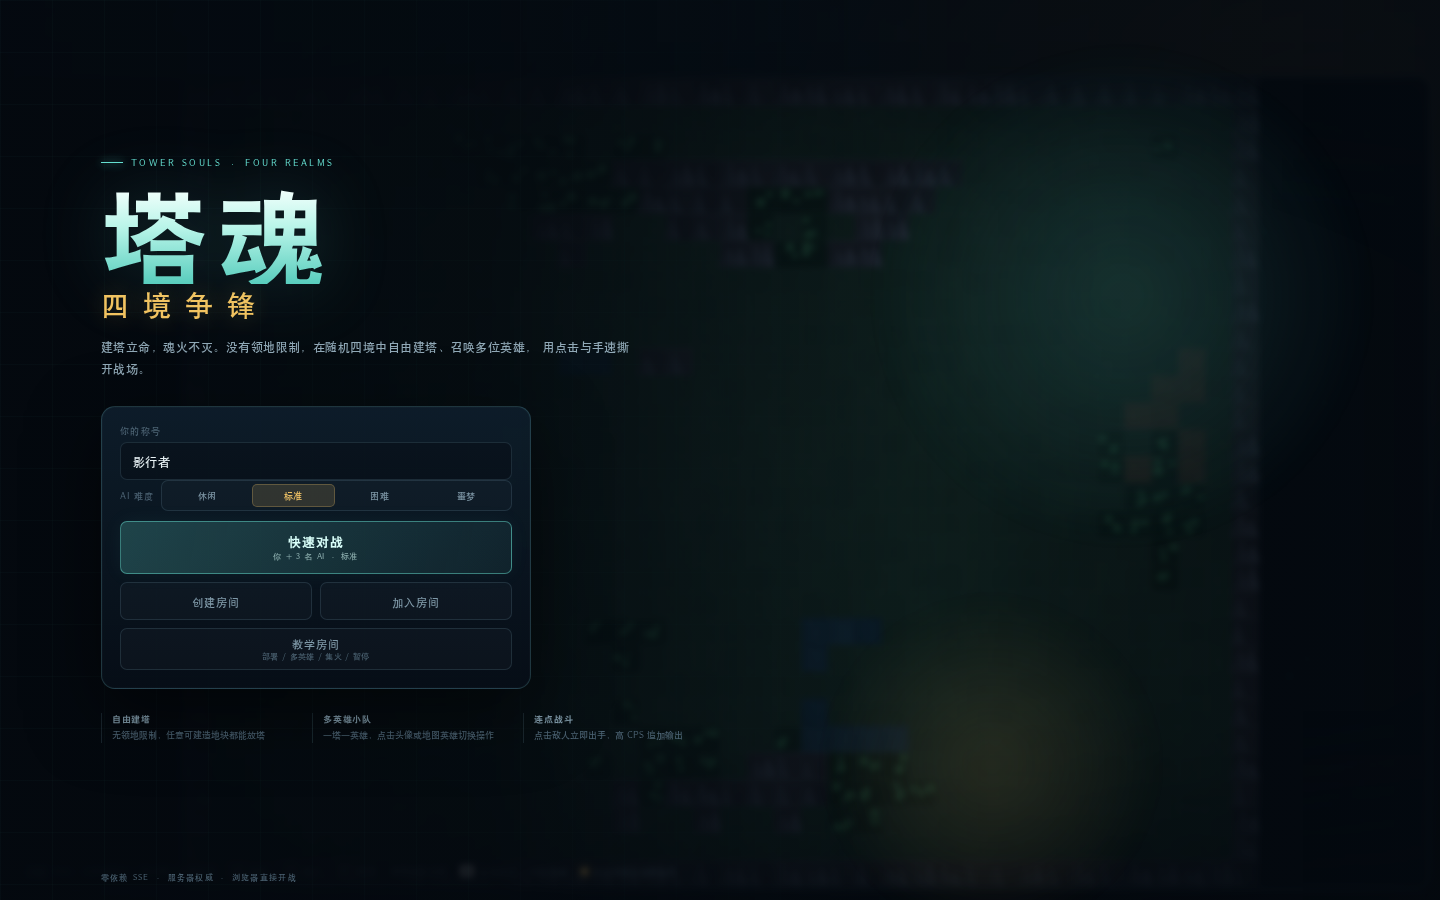
\includegraphics[width=0.92\linewidth,height=0.43\textheight,keepaspectratio]{shots/desktop-start.png}\par
\vfill
{\large 版本 2.12.0 \quad 电脑 + 手机浏览器}\par
\vspace{0.2cm}
{\large\ttfamily http://101.200.74.135:4317}\par
\vspace{0.8cm}
{\color{towersoulsteal}\rule{\linewidth}{1.4pt}}
\end{titlepage}
}
